\usepackage[authoryear,round]{natbib}
\usepackage{multirow}

\newcommand{\sheetnum}{%
	10
}
%\setcounter{section}{\sheetnum-3}
\newcommand{\tutorialtitle}{%
    Locally Linear Embedding (LLE)
}
\newcommand{\tutorialtitleshort}{%
	LLE
}
% for slides
\subtitle{\sheetnum \tutorialtitle}

\maxdeadcycles=1000 % Workaround for ! Output loop---100 consecutive dead cycles because of too many figures

% The following use of algroithms does not work well with the notes:
%
%
%
%
% instead use the following for your algorithms:
%
%\begin{figure}[!t]
%\removelatexerror
%\begin{algorithm}[H]
    % your algo here
    %\label{alg:algolabel}
    %\caption{algocaption}
%\end{algorithm}
%\end{figure}
%\begin{algorithm}
% Below is the definition for the command \removelatexerror:
\makeatletter
\newcommand{\removelatexerror}{\let\@latex@error\@gobble}
\makeatother

\begin{document} %%%%%%%%%%%%%%%%%%%%%%%%%%%%%%%%%%%%%%%%%%%%%%%%%%%%%%%

\sheet{\sheetnum}{\tutorialtitleshort}

\ttopic{\tutorialtitle}

\columnratio{0.2,0.8}\textbf{}
\begin{paracol}{2}
%\setlength{\columnseprule}{0.1pt}
%\setlength{\columnsep}{5em}

\begin{rightcolumn}

% notes version will ignore it
\begin{frame}
\titlepage
\end{frame}

\begin{frame}
\mode<presentation>{
\tableofcontents[hideallsubsections]
}
\mode<article>{
\tableofcontents
}
\end{frame}
\newpage

\mode<all>
\section{Dimensionality reduction revisited}

\begin{frame}{\secname}

\notesonly{
We want to be able to visualize some data that is high-dimensional. We have already encountered approaches for reducing the dimensionality of the data: PCA is one of them. \figref{fig:spiral} 
provides an example of this.
}

\begin{figure}[ht]
     \centering
     \savebox{\imagebox}{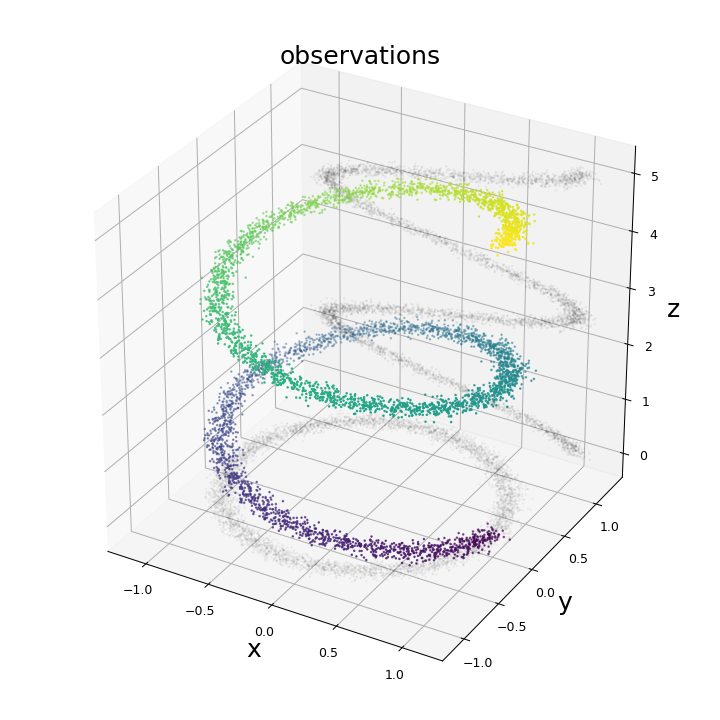
\includegraphics[width=0.4\textwidth]{img/spiral_data.png}}%
     \begin{subfigure}[t]{0.4\textwidth}
         \centering
         \usebox{\imagebox}% Place largest image
         \caption{original observations}
         \label{fig:spiral_data}
     \end{subfigure}
     \hspace{10mm}
     \begin{subfigure}[t]{0.35\textwidth}
         \centering
         \raisebox{\dimexpr.5\ht\imagebox-.5\height}{% Raise smaller image into place
         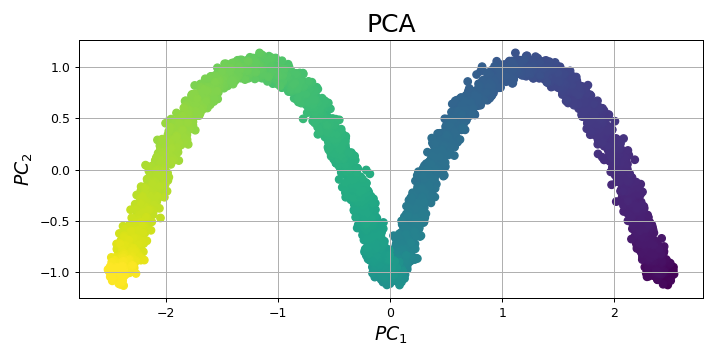
\includegraphics[width=\textwidth]{img/spiral_pca.png}
         }
         \caption{projection onto the first 2 PCs}
         \label{fig:spiral_pca}
     \end{subfigure}
     \notesonly{\caption{Dimensionality reduction of the spiral data using PCA. Points are colored according to their index in the dataset.}}
	 \label{fig:spiral}
\end{figure}


\end{frame}

\section{Global vs. local structure}

\mode<presentation>{
\begin{frame}
	\begin{center}
	
When determining interesting directions in the data, one will either look for ``global'' or ``local'' structure in this data.

	\end{center}
\end{frame}
}

\subsection{The S dataset}

\begin{frame}{\subsecname}


\notesonly{
Let us examine another dataset on which we will also apply PCA\footnote{We will only consider standard linear PCA.} (c.f. \figref{fig:s_data_pca}). The purpose of this is to make the distinction between global and local structure in the data and which type of structure is captured by PCA (the standard linear version of PCA):
}

\begin{figure}[h]
	\centering
    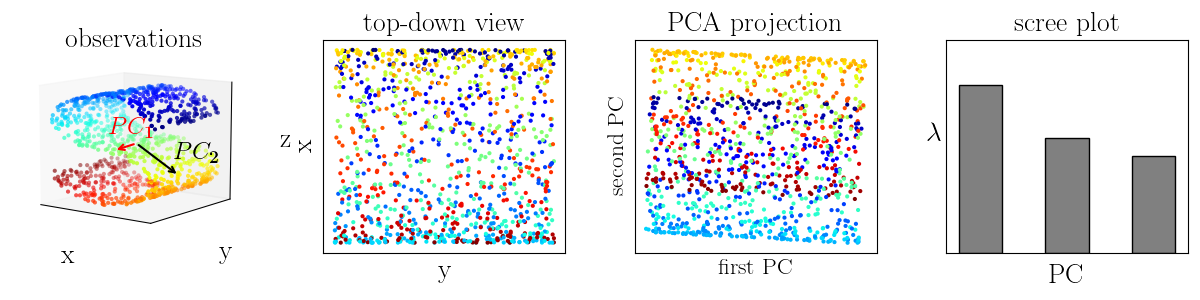
\includegraphics[width=12cm]{img/s_data_pca.png}
	\caption{PCA projection on the ``S'' dataset. Points are colorized according to their index in the dataset.}
	\label{fig:s_data_pca}
\end{figure}

\end{frame}

\notesonly{
Looking at the PCA projections, we recognize that they closely resemble a top-down view of the data. 
The top-down view is effectively a projection of the data onto the xy-plane. The solution found by PCA is one that explains this 3-dimensional \textbf{S} data using a 2D projection such that the variance explained is maximal. The resemblance between the PCA projections and the top-down view tells us that the main ``directions'' in the data are:
\begin{itemize}
\renewcommand\labelitemi{--}
\item \textbf{First}, the direction explained by the PC with highest eigenvalue ($PC_1$):\\
	A crude way of describing it, is that it lies parallel to the original y-axis. It explains the ``thickness'' of the \textbf{S}.
\item \textbf{Second}, the data also follows the direction of the the original x-axis. It is actually slightly tilted. This tilt explains why some color regions appear more narrow on the $PC_2$ axis, than they do in the top-down view.
\end{itemize}

The scree plot tells us how much variance is explained by each principle component. The difference between the last two PCs is less than the difference between either of them and the first PC. 

\question{Why does $PC_1$ explain more variance than either $PC_2$ or $PC_3$?}\\

- The obivous reason is that this is by design. PCA sorts the PCs in order of descending variance ($\corresponds$ eigenvalues). But this is not what we're asking. The question is specific to this \textbf{S}-data. \emph{Why does the PC that lies parallel to the y-axis explain more variance than the PC that lies parallel to the x-axis?} The reason for this is that any point on the $\textbf{S}$ gets  repeated along the y-axis. This three-dimensional $\textbf{S}$ is really a concatenation of multiple ${S}$-curves. The first PC represents which ${S}$-curve a point belongs to. The only thing left to do is to explain \emph{where} we are on a single curve. The second PC is not sufficient to fully describe this with low reconstruction error. We can only achieve a reconstruction error that is sufficiently low if we also take the third PC into account. So the first thing to point out is that PCA does not give us an ideal dimensionality reduction for this dataset. The slight tilt in $PC_2$ is that it only partially describes the $z$ coordinate of a point. We therefore expect that $PC_3$ is needed to fully recover that $z$ coordinate.
}

\begin{frame}
\question{What is PCA doing wrong on the \textbf{S}-data?}

\slidesonly{
\begin{figure}[ht]
	\centering
    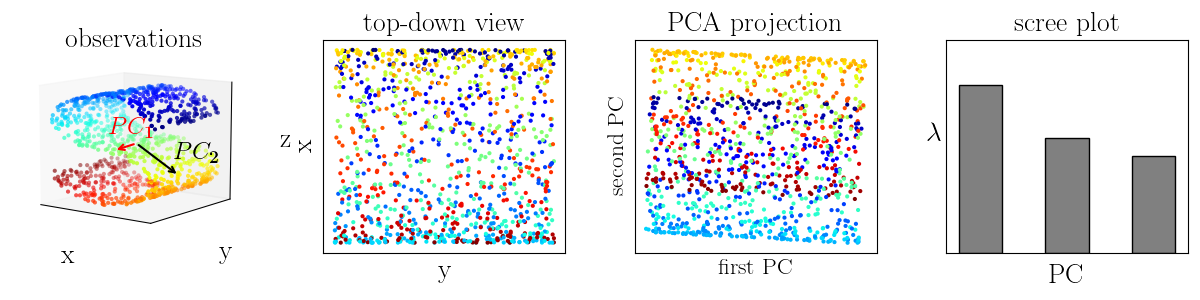
\includegraphics[width=12cm]{img/s_data_pca.png}
	\caption{Comparing PCA projections with embedding solutions. Points are colorized according to their index in the dataset.}
	\label{fig:s_data_pca}
\end{figure}
}

\notesonly{
- The points were colored according to the order in which they appear in the dataset. PCA does not account for this order. Shuffling the order of the samples leads to the exact same PCs. Nonetheless, we recognize that each group of similarly colored points share proximity to one another. To be more specific: Points with the same color lie on the same location on two different ${S}$-curves. So color represents the position on a curve and that position can only be described by the remaining two PCs. When we look at the PCA projection, we also recognize that colors overlap, specifically Blue, Green and and Red. Those three colors represent different elevation levels on the $\textbf{S}$. \emph{Is this overlap a bad thing?} They have something in common, so we want them to appear closer to one another. So let us look at what the PCA projections tell us about the color groups:


\begin{itemize}
\renewcommand\labelitemi{--}
\item \textcolor{red}{Red} is closer to \textcolor{blue}{Blue} than it is to \colorbox{yellow}{Yellow}. Looking at $PC_2$ confirms this.
\item \textcolor{red}{Red}, \textcolor{blue}{Blue} and \textcolor{green}{Green} are close to one another. Looking at $PC_2$ confirms this also. However, it does not reveal that \textcolor{red}{Red} is actually \textbf{closer} to {\color{green}{Green}}, than it is to \textcolor{blue}{Blue}.
\end{itemize}
}
\end{frame}

\notesonly{
What is missing from PCA is that it doesn't prioritize that this $\textbf{S}$ is made up from multiple ${S}$-curves stacked next to each other. Knowing this information enables to find a much more compact representation for describing the data. One might actually find it completly irrelevant that the data describes resembles an $\textbf{S}$ and by doing so, one could find a more compact representation for the data. This is done by finding a representaiton that focus on preserving local structure.

PCA is designed to find ``global'' structure in the data. It does not restrict itself to preserving local structure. The colors show us the local structure in the data and we no longer recognize this in the PCA projections. Clustering methods base their structure on proximity measures. The proximity can be measured between a point and other data points (e.g. pairwise clustering). Clustering reveals more information about local structure than it does about global structure (i.e. the index/label assigned to a cluster is arbitrary).
}

\question{What about ICA?}\\

- The independence assumption in ICA also enables it to find local structures.

This is not to make the point that linear PCA is not an effective method for dimensionality reduction. This is \textbf{not} the takeaway from all this is. The point is to know that linear PCA attends to global structure and that the user needs to decide whether they are actually interested in global or local structures. Do we care about where we are on an $S$-curve or not?


\begin{frame}
\question{What do we mean when we talk about \emph{global} and \emph{local} structures in the data?}\\

\notesonly{
- Pick any two neighboring points from some dataset. Their proximity to one another lets us assume they have more in common than a pair of points that are far away from one another \footnote{This proximity assumption forms the basis for pairwise clustering.}. If we perform PCA on this data and project it onto the principle components, we may find that the two points that were neighbors in the original space are no longer neighbors in the space spanned by the PCs. To be more precise, if their projections do happen to appear close to one another, then this is due to the linearity in the data. But what about non-linear manifolds? PCA does not try to preserve any neighborhood or ``local'' information. This becomes a problem if the ``local'' information is key to \emph{efficiently} reduce the dimensionality.
}

\begin{figure}[ht]
	\centering
	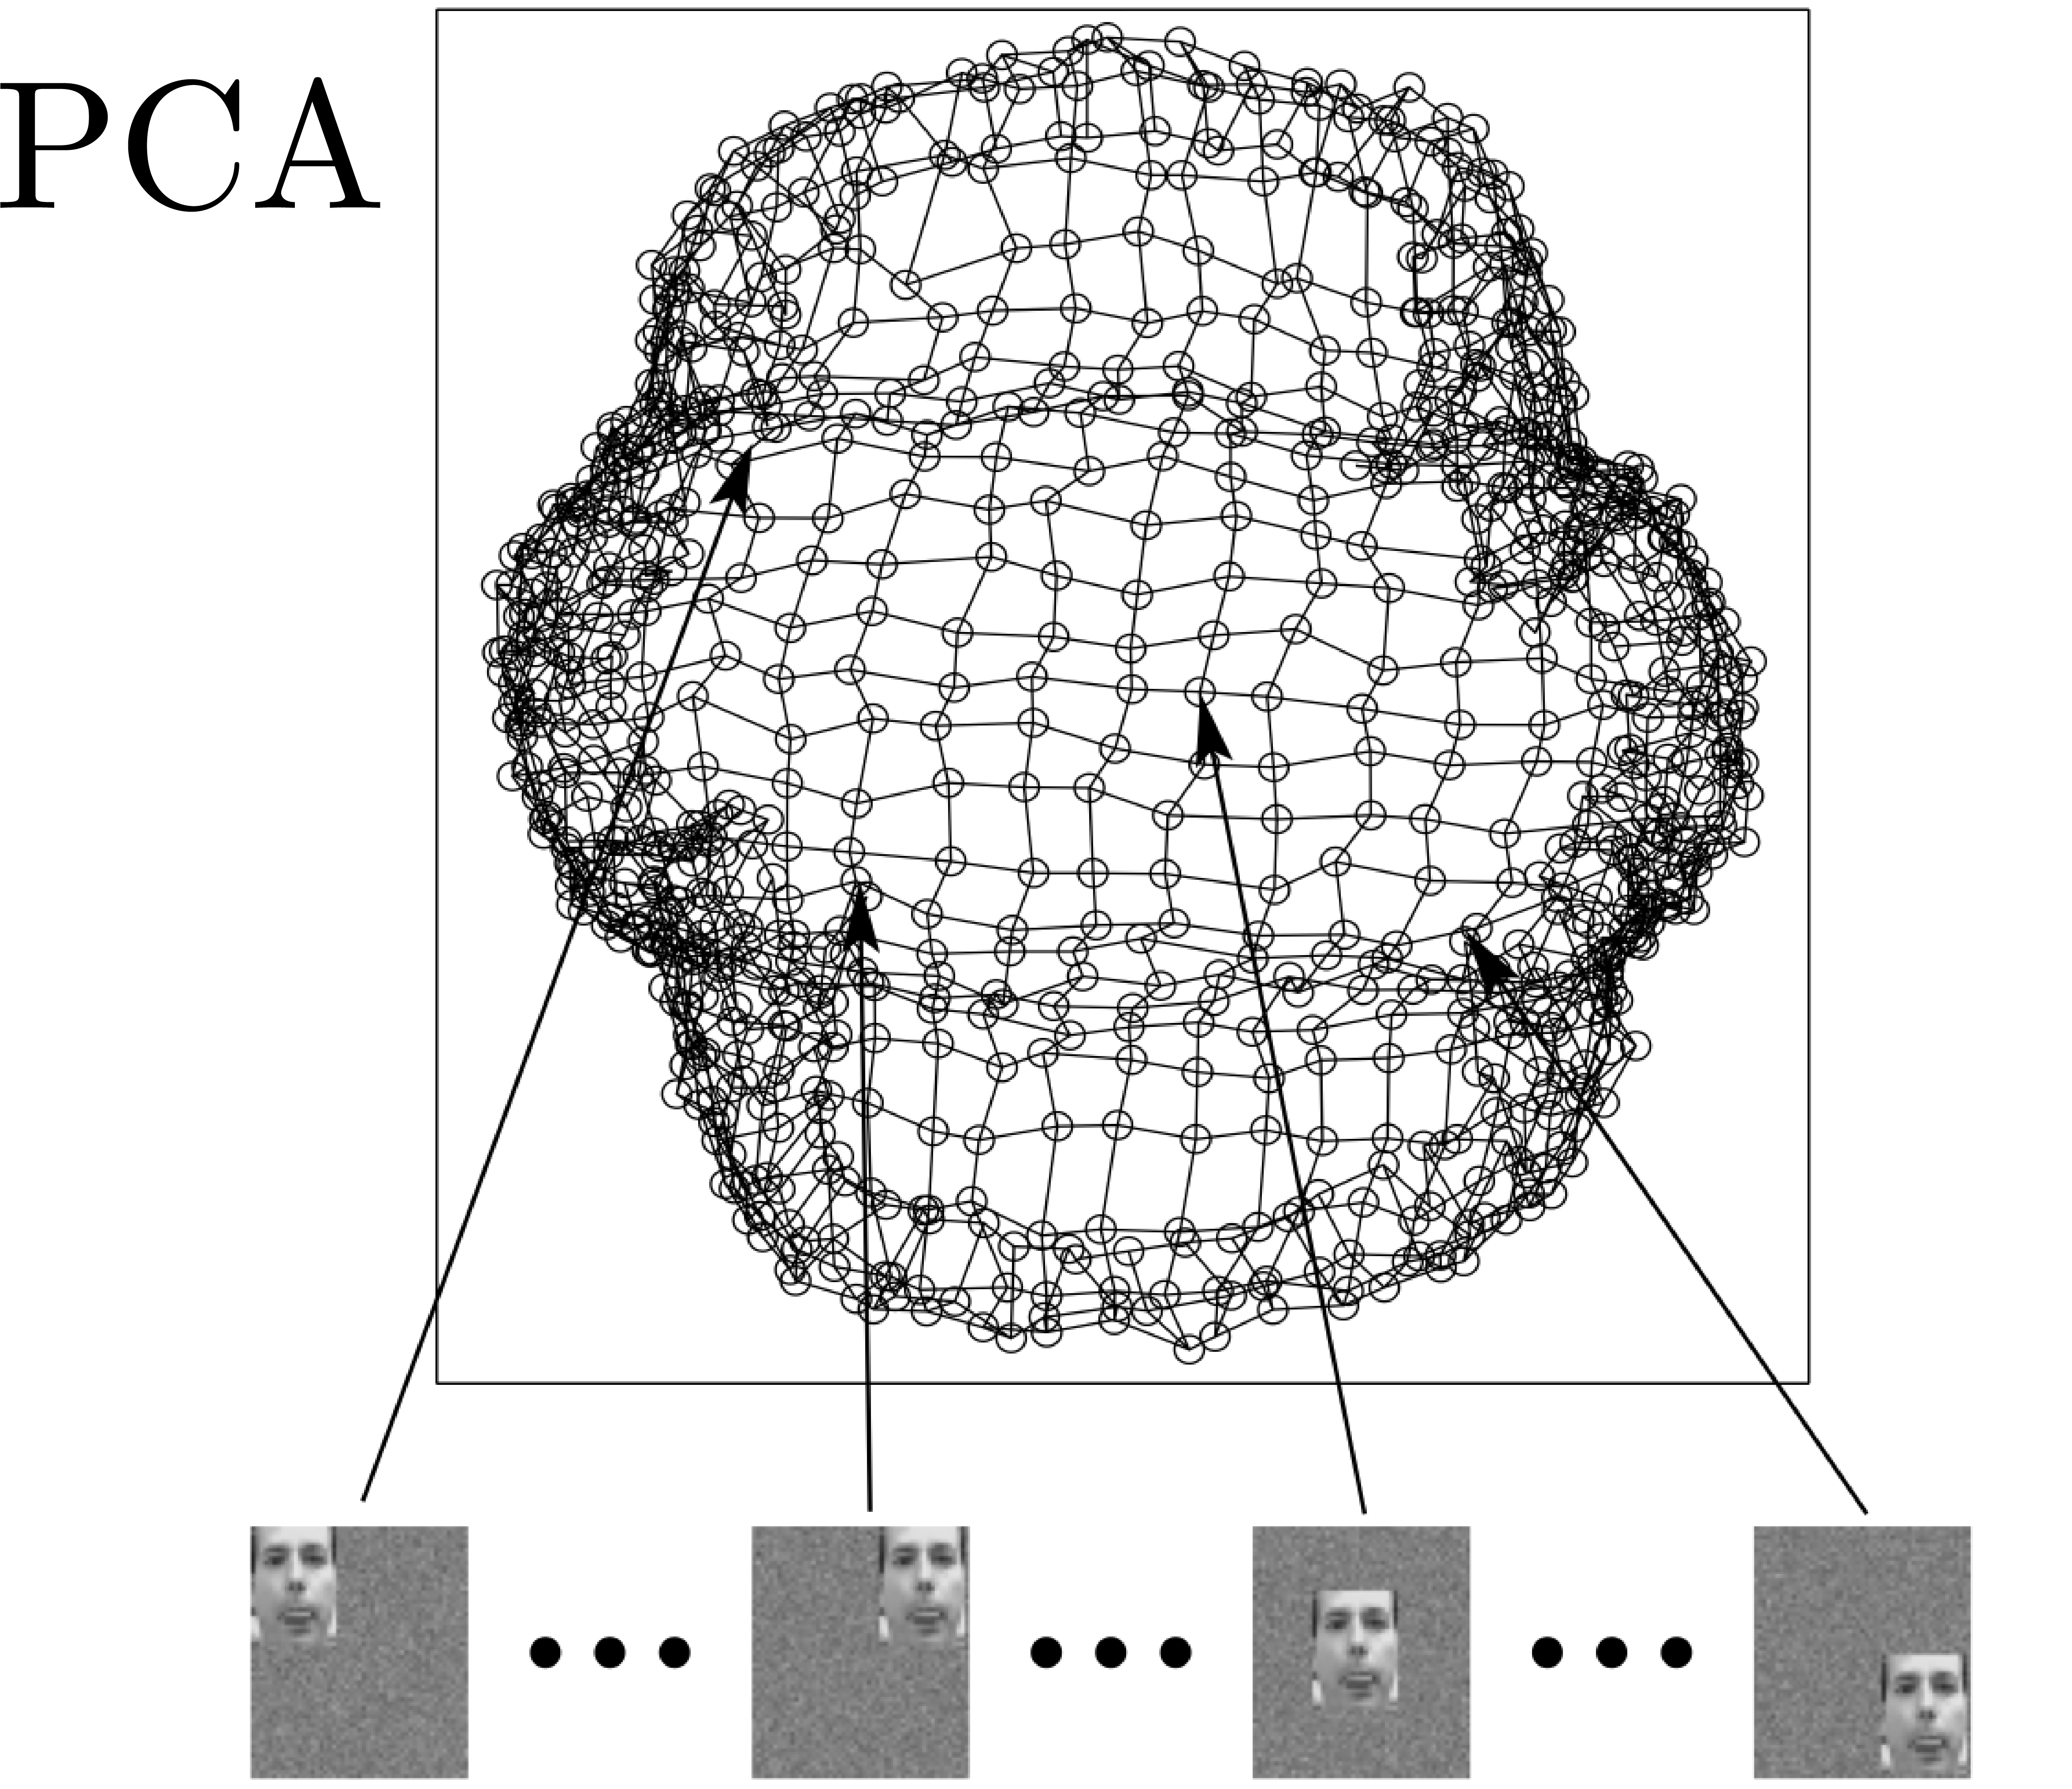
\includegraphics[width=4.3cm]{img/fig3_lle_intro_cropped_pca.png}
	\caption{PCA projections of translated versions of the same image}
	\label{fig:faces_translated_pca}
\end{figure}

\question{What are the 2-d coordinates of the face if it is shifted to the bottom-left corner?}

\end{frame}


Consider the images in \figref{fig:faces_translated_pca}. The data consists of images where a \textbf{single} picture of a face surrounded by some noisy background. Each image shows the face picture at a different location within the image. The images are projected onto the space spanned by the first two PCs. We examine the projections due to moving the face from one corner to another and find that no relation between the coordinates of the projection and the translation applied to the face picture. If we wanted to predict the coordinates of an image where the face is shifted to the bottom left corner, we wouldn't be able to make that prediction.


\mode*

\clearpage

\mode<all>
\section{Locally Linear Embedding (LLE)}

\mode<presentation>{
\begin{frame} 
    \begin{center} \huge
        \secname
    \end{center}
\end{frame}
}

\subsection{Motivation}

\begin{frame}{\subsecname}

Find structure in the data that extends to non-linear manifolds.

\notesonly{

$\textbf{S}$-dataset provides an example of a non-linear manifold.}

\begin{figure}[ht]
	\centering
    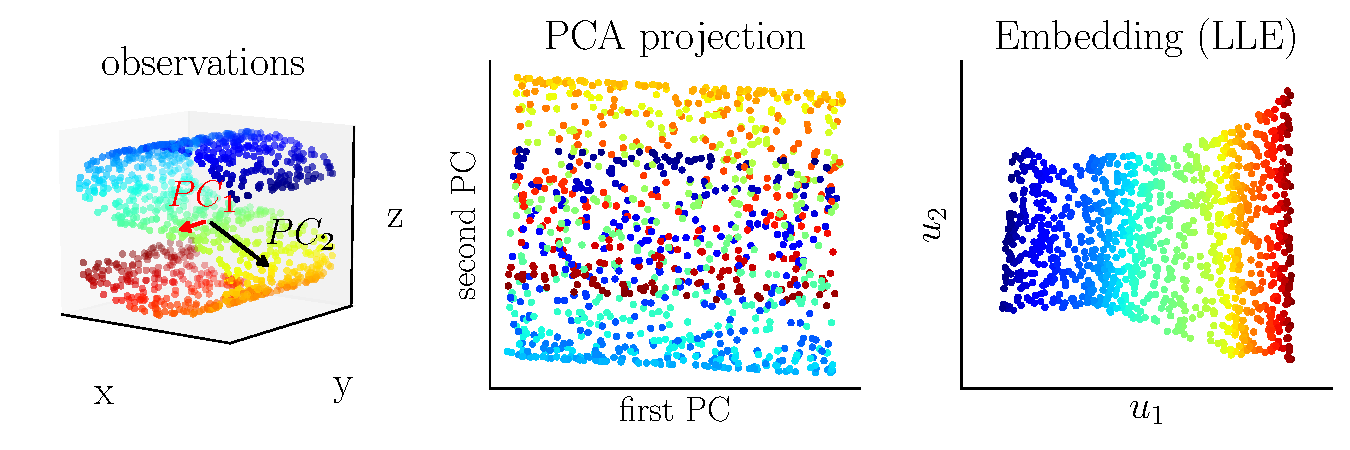
\includegraphics[width=12cm]{img/s_data_proj}
	\notesonly{\caption{The S-dataset, PCA projections and embedding solution. Points are colorized according to their index in the dataset.}}
	\label{fig:s_data_proj_lle}
\end{figure}

\notesonly{
Utilize this to r}\slidesonly{R}educe the dimensionality of the data such that points that lie close \textbf{on} the manifold also lie close in their projection\notesonly{ (we will refer to the projection space which preserving local neighborhoods / ``structure preserving'' as \emph{embedding space})}.

\end{frame}

\notesonly{
Looking at \figref{fig:s_data_proj_lle} we see that the nonlinear manifold is preserved in the LLE embedding, while PCA does not capture the non-linear local structure. The same can be said for \figref{fig:faces_translated_pca_lle}, translating the images from one corner to another has a corresponding translation in the embedded space. In this case we can also infer the coordinates of an image where the face appears in the bottom-left corner in the embedded space.
}

\begin{frame}
\slidesonly{
 \frametitle{PCA vs. Locally Linear Embedding (LLE)}
}

\svspace{-5mm}
 
\begin{figure}[ht]
	\centering
    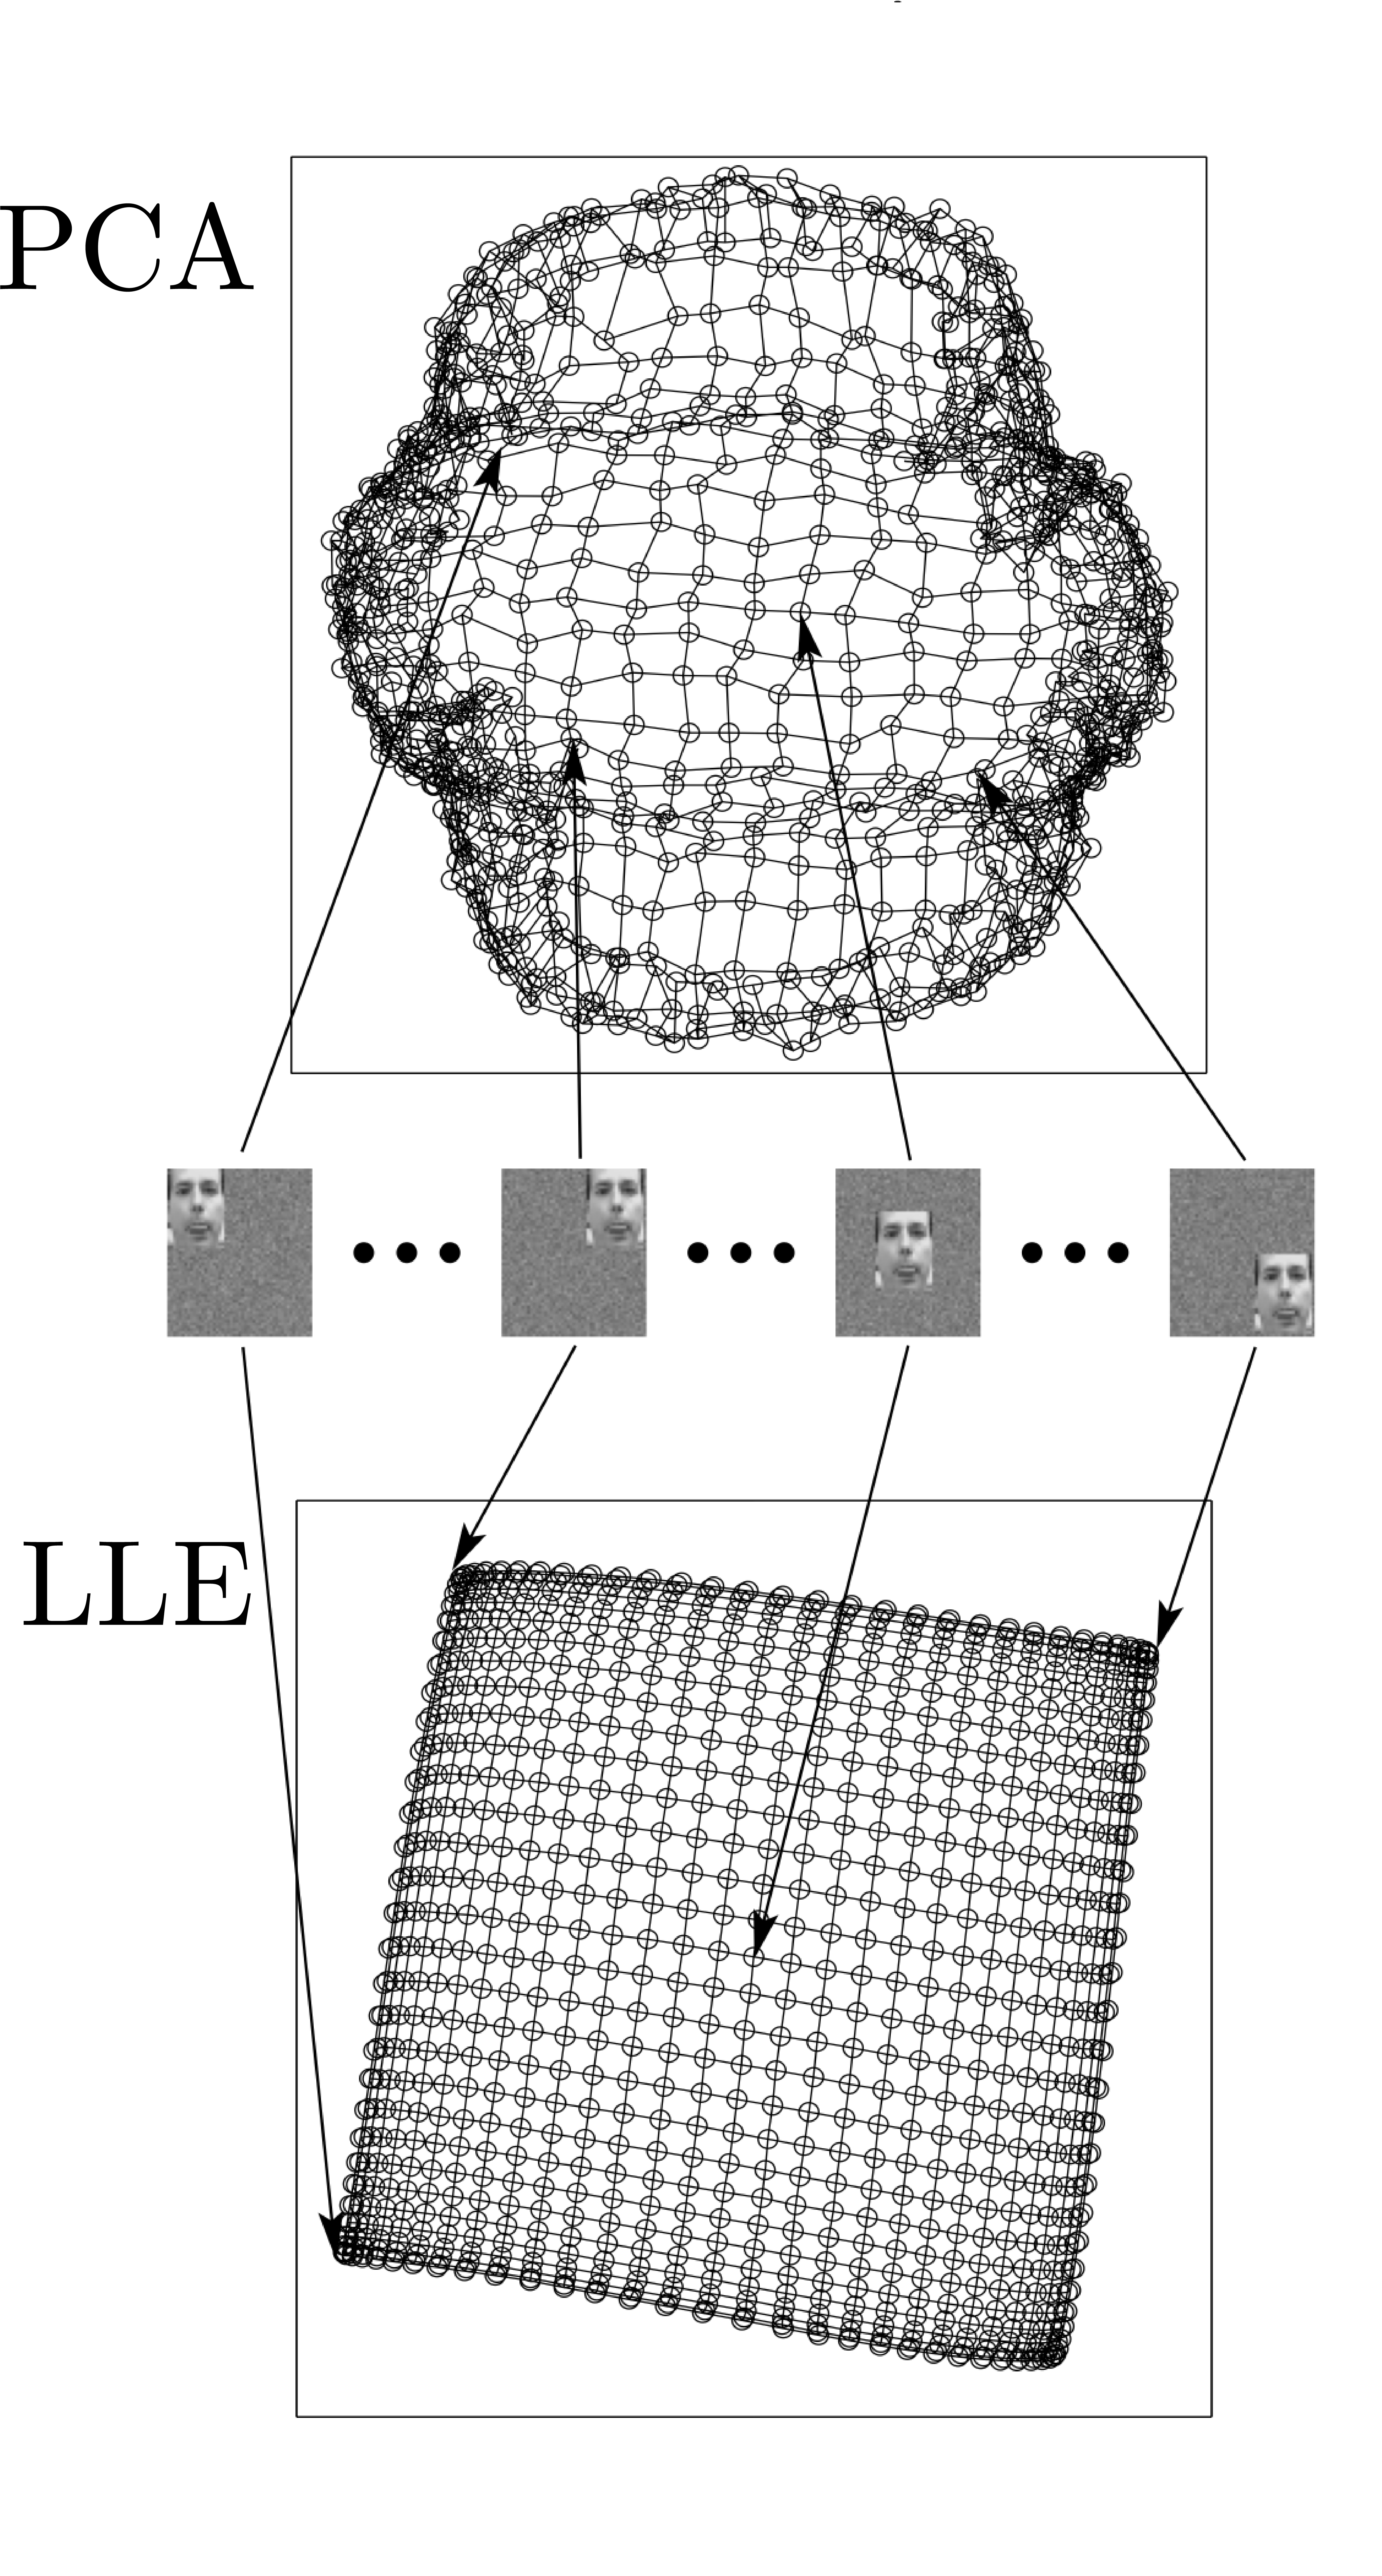
\includegraphics[width=0.3\textwidth]{img/fig3_lle_intro_cropped.png}
	\caption{PCA projections and LLE of translated versions of the same image. What would be the coordinates of the face-in-bottom-left-corner-image be?}
	\label{fig:faces_translated_pca_lle}
\end{figure}
\end{frame}

\subsection{Algorithm outline}

\subsubsection{A representation of local structure}

\begin{frame}{\subsecname:~\subsubsecname}

\notesonly{
LLE is a fairly simple algorithm. }Local structure is preserved by optimizing the projection of a neighborhood of points (PCA finds a projection for all points collectively).

\pause

But first we have to identify the neighborhood.

\end{frame}

\begin{frame}{\subsecname:~\subsubsecname}

\question{How do we ``localize'' the local structure?}

\pause

- through K-nearest neighbors (KNN)

\begin{center}
    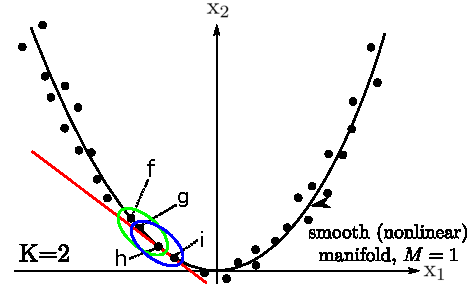
\includegraphics[width=0.6\textwidth]{img/section4_fig11_K2}
    \captionof{figure}{Finding the projection of a neighborhood of points.}
	\label{fig:tangentialk2}
\end{center}

\end{frame}

\begin{frame}{\subsecname:~\subsubsecname}

\slidesonly{
\begin{center}
    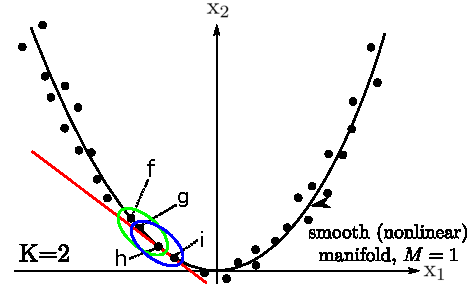
\includegraphics[width=0.5\textwidth]{img/section4_fig11_K2}
    \captionof{figure}{Finding the projection of a neighborhood of points.}
	\label{fig:tangentialk2}
\end{center}
}
\only<1>{
\question{What do we do with the KNN?}
}

\only<2>{
\notesonly{

- We approximate each point as a weighted sum of its KNN.
}
\begin{equation}
\vec{x}^{(\alpha)} \approx \hspace{-3mm} \sum_{\beta \in \operatorname{KNN}(\vec{x}^{(\alpha)})}^{} \hspace{-5mm} \mathrm{W}_{\alpha \beta} \cdot \vec{x}^{(\beta)} \qquad \forall \; \alpha
\end{equation}

The first thing to optimize in LLE are the reconstruction weights $W_{\alpha\beta}$ to yield a good approximation of $\vec x^{(\alpha)}$
}

\end{frame}

\begin{frame}{Optimizing the reconstruction weights}

\begin{align}
\only<1->{
\vec{x}^{(\alpha)} &\approx \hspace{-3mm} \sum_{\beta \in \operatorname{KNN}(\vec{x}^{(\alpha)})}^{} \hspace{-5mm} \mathrm{W}_{\alpha \beta} \cdot \vec{x}^{(\beta)} &\qquad \forall \; \alpha
}
\only<2->{
\intertext{A good approximation is one with minimal squared Euclidean distance:}
\Big\lVert \vec{x}^{(\alpha)} &- \hspace{-3mm} \sum_{\beta \in \operatorname{KNN}(\vec{x}^{(\alpha)})}^{} \hspace{-5mm} \mathrm{W}_{\alpha \beta} \cdot \vec{x}^{(\beta)} \Big\rVert_2^2 \eqexcl \min_{\{W_\alpha\beta\}} &\qquad \forall \; \alpha
}
\end{align}

Next,
\begin{itemize}
\item Formulate a cost function for finding a good approximation for all points $\alpha=1,\ldots,p$ in the dataset,
\item also, store the reconstruction weights into a matrix $\vec W$
\item add constraints
\end{itemize}

\end{frame}

\begin{frame}{Calculate the reconstruction weights}

\begin{align}
E(\vec{W}) =& \sum_{\alpha=1}^{p} \overbrace{\Big\lVert{\vec{x}^{(\alpha)} - \sum_{\beta=1}^{p} \mathrm{W}_{\alpha \beta} \vec{x}^{(\beta)}}\Big\rVert_2^2}^{\substack{\text{reconstruct } \vec{x}^{(\alpha)} \text{ by its } \\ K \text{ nearest neighbors only}}} \;\; \eqexcl \;\; \min_{\vec W}\\
\text{s.t.} \quad &\mathrm{W}_{\alpha \beta} = 0 \text{ if } \beta \notin \operatorname{KNN}(\vec{x}^{(\alpha)}), \\
&\sum_{\beta=1}^{p} \mathrm{W}_{\alpha \beta} = 1 \;\; \text{(The neighborhood has to ``explain'' the point)}
\end{align}



\end{frame}

\begin{frame}{Properties of the reconstruction weights}

\svspace{-5mm}

\slidesonly{
\begingroup
\footnotesize
\begin{align}
E(\vec{W}) =& \sum_{\alpha=1}^{p} \overbrace{\Big\lVert{\vec{x}^{(\alpha)} - \sum_{\beta=1}^{p} \mathrm{W}_{\alpha \beta} \vec{x}^{(\beta)}}\Big\rVert_2^2}^{\substack{\text{reconstruct } \vec{x}^{(\alpha)} \text{ by its } \\ K \text{ nearest neighbors only}}} \;\; \eqexcl \;\; \min_{\vec W}\\
\text{s.t.} \quad &\mathrm{W}_{\alpha \beta} = 0 \text{ if } \beta \notin \operatorname{KNN}(\vec{x}^{(\alpha)}), \\
&\sum_{\beta=1}^{p} \mathrm{W}_{\alpha \beta} = 1 \;\; \text{(The neighborhood has to ``explain'' the point)}
\end{align}
\endgroup
}

\svspace{-5mm}

\begin{minipage}{0.25\textwidth}
\begin{center}
	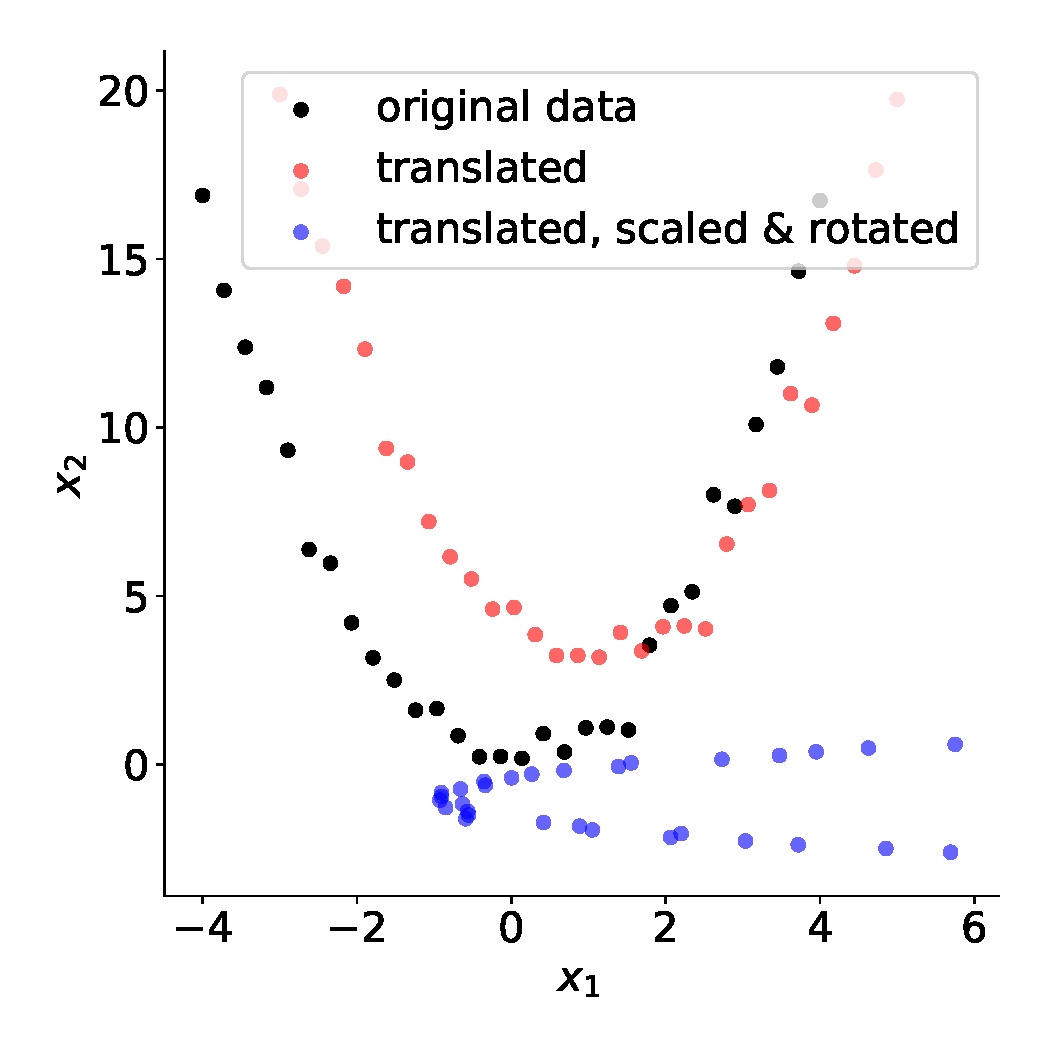
\includegraphics[width=1.2\textwidth]{img/parabola_data}
	\notesonly{\captionof{figure}{2D points describing a parabola.}}
\end{center}
\end{minipage}
\hspace{2mm}
\begin{minipage}{0.7\textwidth}
\begin{center}
	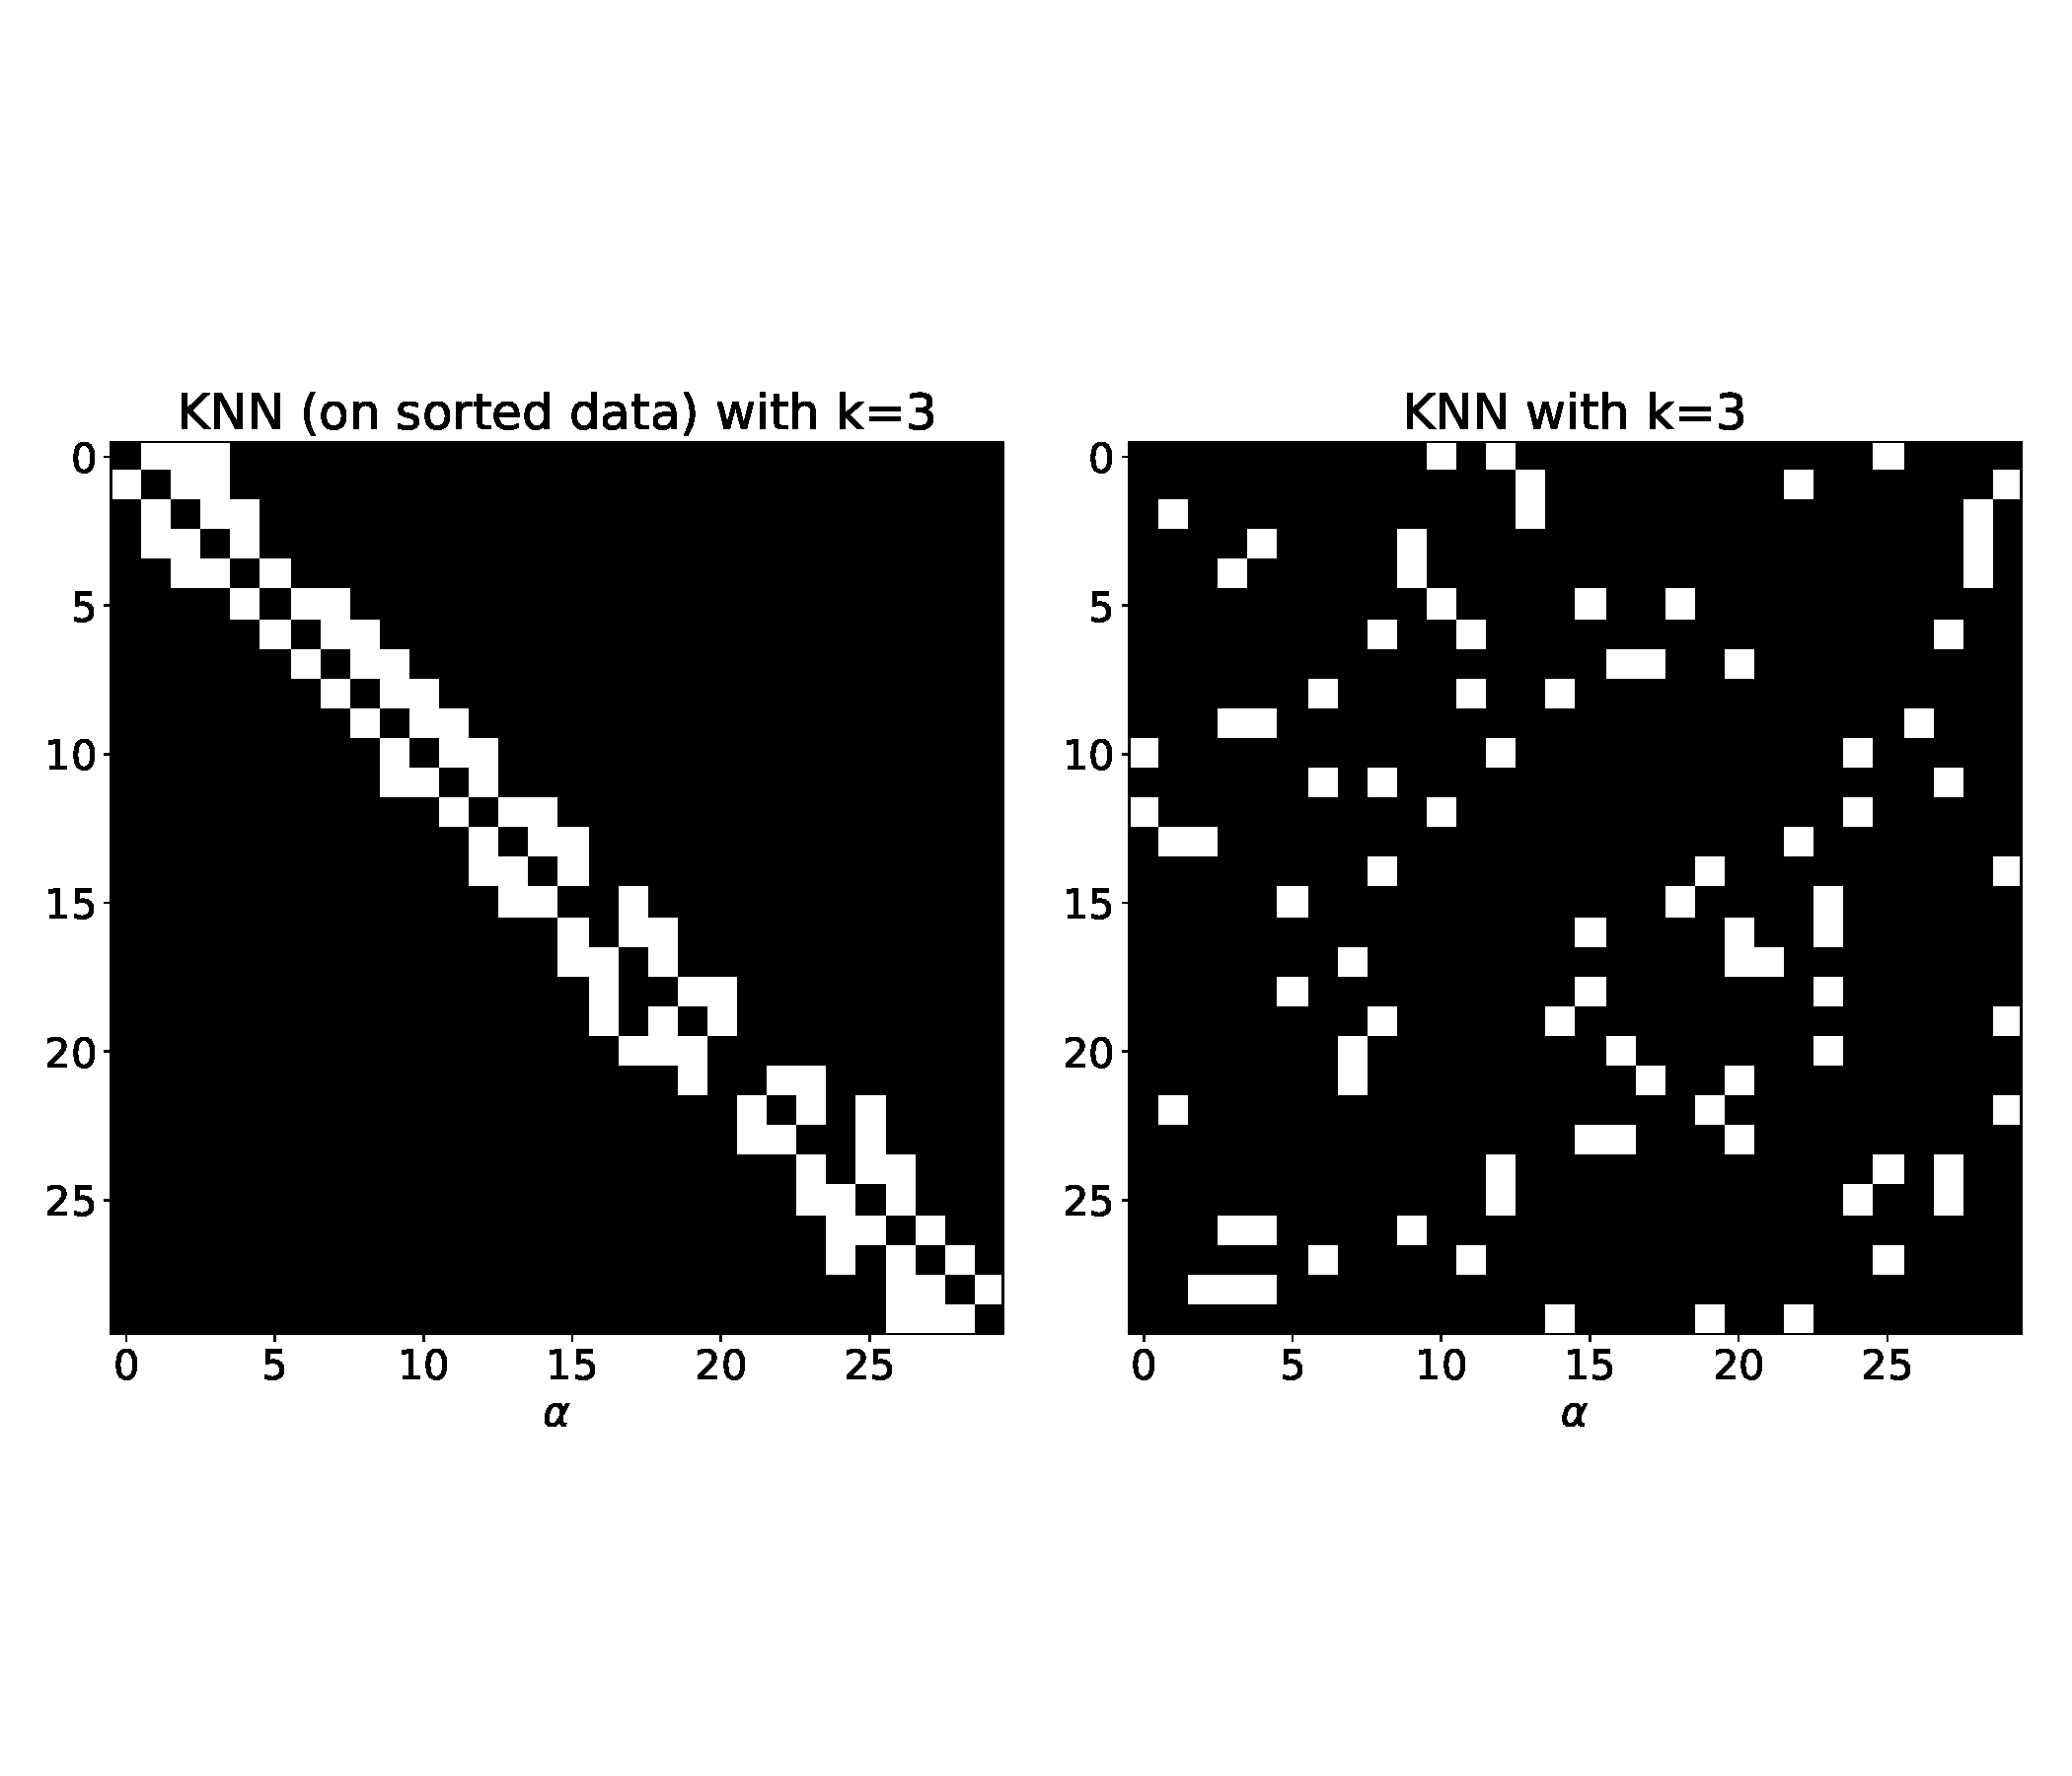
\includegraphics[trim=0 180 0 180, clip, width=0.92\textwidth]{img/parabola_knn}
	\notesonly{\captionof{figure}{Highlighting the KNN.}}
\end{center}
\end{minipage}

\end{frame}

\subsubsection{The embedding coordinates}

\begin{frame}{\subsubsecname}

Local structure is now stored in the reconstruction weights $\vec W$.

We have used $\vec W$ to reconstruct any point $\vec x^{(\alpha)}$ in the input space $\R^N$.

The embedding space has to preserve the local structure.

If the embedding space maps every point $\vec x^{(\alpha)}$ to an $M$-dimensional space with 
coordinates $\vec u^{(\alpha)} \in \R^M$, then the following approximation:

\begin{equation}\vec{u}^{(\alpha)} \approx \hspace{-3mm} \sum_{\beta \in \operatorname{KNN}(\vec{x}^{(\alpha)})}^{} \hspace{-3mm} \mathrm{W}_{\alpha \beta} \cdot \vec{u}^{(\beta)}
\end{equation}

should hold as well.

\end{frame}

\begin{frame}{Finding the embedding coordinates}

The reconstruction weights in $\vec W$ remain \emph{fixed}.

The embedding coordinates are found by minimizing the approximation error of every point $\vec u^{(\alpha)}$ through its local neighborhood:

\begin{equation}
	F(\vec U) =
    \sum_{\alpha=1}^{p} 
	\bigg(  \vec{u}^{(\alpha)}  - \sum_{\beta=1}^{p} W_{\alpha \beta} \vec{u}^{(\beta)}
	\bigg) ^ 2
\end{equation}

where $\vec U \in \R^{M,p}$ is the embedded dataset with all $p$ points.

\end{frame}


\begin{frame}
The binomial expansion leads to an equivalent formulation of the cost function as:

\svspace{-5mm}

\begin{align}
F(\vec{U}) =& 
\sum_{\alpha, \beta=1}^{p}
\Big\lbrack
\delta_{\alpha \beta} - \mathrm{W}_{\alpha \beta} - \mathrm{W}_{\beta \alpha} + \sum_{\gamma=1}^{p} \mathrm{W}_{\gamma \alpha} \mathrm{W}_{\gamma \beta} \Big\rbrack (\vec{u}^{(\alpha)})^\top \vec{u}^{(\beta)} \\
=& \sum_{\alpha, \beta=1}^{p} g_{\alpha \beta} (\vec{u}^{(\alpha)})^\top \vec{u}^{(\beta)}
\end{align}

\question{What do we expect for the embedding coordinates?}

\pause

\svspace{-3mm
}
\begin{itemize}
\item[-] Translation, scaling and rotation of the original dataset $\vec X$ should yield the same embedding coordinates $\vec U$.
\item[-] The above invariances are already properties of the reconstruction weights $\vec W$.
\item[-] Minimizing the squared Euclidean distance enables the above invariances.
\item[-] We still have to prevent the trivial solution of $\vec u^{(\alpha)} = \vec 0 \;\; \forall \;\; \alpha$
\end{itemize}

\end{frame}



\mode<article>{
%\begin{frame}%[label=g_alpha_beta_proof]{Supplementary Material}
%\begin{textblock}{5}(13,0.075)
	%\hyperlink{g_alpha_beta_slide}{\beamerbutton{back to lecture}}
%\end{textblock}
	Derivation of $g_{\alpha \beta}$ in the cost function
	$F(\vec U) =
    \sum_{\alpha=1}^{p} 
	\bigg(  \vec{u}^{(\alpha)}  - \sum_{\beta=1}^{p} W_{\alpha \beta} \vec{u}^{(\beta)}
	\bigg) ^ 2
    $ 
    for finding the optimal embedding coordinates.\\
    First, a brief refresher on binomial expansion of vectors:
	%{\footnotesize{}
    \begin{align}
    \big( 
		\vec{a}
		- \vec{b}
	\big) ^ 2 
    &= \big(  \vec{a} - {\color{blue}\vec{b}} \big)^\top \big(  \vec{a} - {\color{red}\vec{b}} \big)\\
    &= \vec a^\top \vec a 
    - \vec a^\top {\color{red}\vec{b}}
    - {\color{blue}\vec{b}^\top} \vec a 
    - {\color{blue}\vec{b}^\top} {\color{red}\vec{b}}
    \end{align}\\
    
    Let $\;\vec a = \vec u^{(\alpha)}\;$ and 
    $\;{\color{red}
    \vec{b}=\sum_{\beta=1}^{p} W_{\alpha \beta} \vec{u}^{(\beta)}
    } \Leftrightarrow {\color{blue}
    \vec{b}^{\top}=\sum_{\beta=1}^{p} 
    W_{\beta \alpha} \left(\vec{u}^{(\beta)}\right)^\top
    }
    $
    
    \question{Why do we flip the indices from 
    ${\color{red} W_{\alpha \beta}}$ to ${\color{blue} W_{\beta \alpha}}$?}\\
    The reason we flip the Transposing $\vec u^{(\beta)}$ 
    
    \begin{align}
	= &\sum_{\alpha=1}^{p} 
	\bigg[ 
	(\vec{u}^{(\alpha)})^2
	- 2 \sum_{\beta=1}^{p} W_{\alpha \beta} (\vec{u}^{(\alpha)} )^\top \vec{u}^{(\beta)}
	+
	\sum_{\beta=1, \gamma=1}^{p} W_{\alpha \beta} W_{\alpha \gamma} (\vec{u}^{(\beta)} )^\top \vec{u}^{(\gamma)}
	\bigg]
	\\
	= &\sum_{\alpha=1}^{p} 
	\bigg[ 
	(\vec{u}^{(\alpha)})^2
	- \sum_{\beta=1}^{p} W_{\alpha \beta} (\vec{u}^{(\alpha)} )^\top \vec{u}^{(\beta)}
	- \sum_{\beta=1}^{p} W_{\beta \alpha} (\vec{u}^{(\beta)} )^\top \vec{u}^{(\alpha)}
	\\~~~~~~~&+
	\sum_{\beta=1}^{p} 
		\sum_{\gamma=1}^{p} 
		\bigg(
			W_{\gamma \alpha} 
			W_{ \gamma \beta}
		\bigg) 
		(\vec{u}^{(\alpha)} )^\top \vec{u}^{(\beta)}
	\bigg]
	\\
	= &\sum_{\alpha, \beta=1}^{p} 
	\bigg\{ \underbrace{
		\delta_{\alpha \beta}
		- W_{\alpha \beta}
		- W_{\beta \alpha}
		+
		\sum_{\gamma=1}^{p} 
			W_{\gamma \alpha} W_{\gamma \beta} }_{=g_{\alpha \beta}}
	\bigg\}
	(\vec{u}^{(\alpha)} )^\top \vec{u}^{(\beta)}
	\end{align}
    %}
%\end{frame}
}

\begin{frame}{A constrained optimization problem}

minimize $F(\vec{U}) = \sum_{\alpha, \beta=1}^{p} g_{\alpha \beta} (\vec{u}^{(\alpha)})^\top \vec{u}^{(\beta)}$
\begin{align}
\quad \text{s.t.} \quad
%&\sum_{\alpha=1}^{p} \vec{u}^{(\alpha)} = 0,\quad \text{(remove translation freedom)} \\
&\frac{1}{p} \sum_{\alpha=1}^{p} \vec{u}^{(\alpha)} (\vec{u}^{(\alpha)})^\top = \vec{I} \quad \text{(prevent trivial solution } \vec{u}^{(\alpha)} = \vec{0})
\end{align}

\end{frame}

\begin{frame}

Reformulating $F(\vec U)$ may provide intuition to finding the embedding coordinates $\vec U$:

\begingroup
\small
\begin{align}
\intertext{with $\sum_{\alpha, \beta=1}^{p} g_{\alpha \beta} u_i^{(\alpha)} u_i^{(\beta)}$}
F(\vec U) =& \sum_{i=1}^M \sum_{\alpha, \beta=1}^{p} g_{\alpha \beta} u_i^{(\alpha)} u_i^{(\beta)}
\intertext{and having all $\{g_\alpha\beta\}$ stored in a matrix $\vec G = \Big( \vec{I} - \vec{W}^\top \Big) \Big( \vec{I} - \vec{W} \Big)$ we can rewrite $F(\vec U)$ as}
=& \sum_{i=1}^M  \vec u_{(i)}^\top \vec G \, \vec u_{(i)} = 
\sum_{i=1}^M \vec u_{(i)}^\top \vec u_{(i)} \lambda_{i}
\end{align}
\endgroup

\end{frame}

\begin{frame}

\slidesonly{
\begin{equation}
F(\vec U)
= \sum_{i=1}^M  \vec u_{(i)}^\top \vec G \, \vec u_{(i)} = 
\sum_{i=1}^M \vec u_{(i)}^\top \vec u_{(i)} \lambda_{i}
\end{equation}

Recall from PCA:
\begin{equation}
	\underbrace{ \vec{e}_a^\top \vec{C} \, \vec{e}_a }_{
		\text{objective} }
	- \lambda \underbrace{ \big( \vec{e}_a^\top\vec{e}_a - 1 \big) }_{
			\text{constraints} }
	\eqexcl \max
\end{equation}
}

Finding $\vec U$ involves finding the eigenfunctions of $\vec G$.

\begin{equation}
\vec G \vec e_j = \lambda_j \vec e_j
\end{equation}

\question{Which eigenvectors do we look for?}

\notesonly{
-Unlike PCA, which tries to maximize the Lagrangian, we're trying to minimize $F(\vec U)$.
Therefore, we will be looking for the eigenvectors with \emph{smallest} eigenvalues.

Local structure is described by the eigenvectors with small eigenvalues.

In order to obtain $M$ embedding coordinates, we find the $M+1$ eigenvectors with smallest eigenvalues and discard the last eigenvector. In this case the last eigenvector will always be associated with a $\lambda$ of zero, so there's no information about the manifold there.
}
\end{frame}

\subsection{Remarks}

\begin{frame}{Remarks}


\begin{minipage}{0.47\textwidth}
\begin{center}
	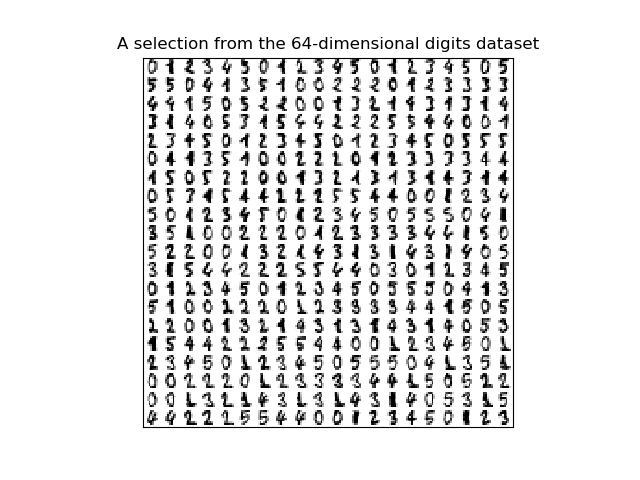
\includegraphics[width=0.9\textwidth]{img/digits}
	\notesonly{\captionof{figure}{Digits data.}}
\end{center}
\end{minipage}
\begin{minipage}{0.47\textwidth}
\begin{center}
	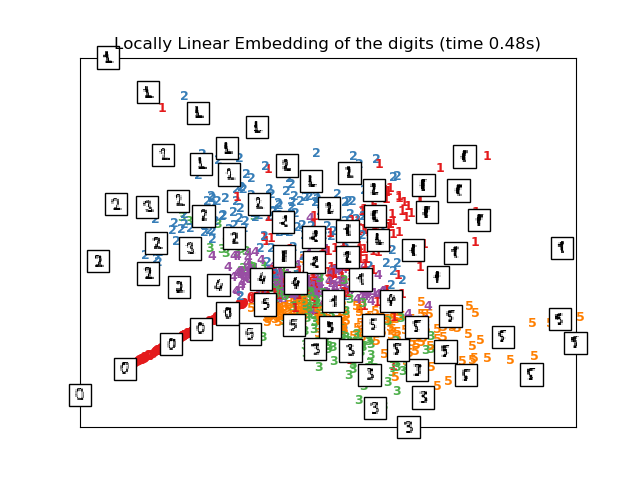
\includegraphics[width=0.95\textwidth]{img/digits_lle}
	\notesonly{\captionof{figure}{2D Embedding of the digits data using LLE.}}
\end{center}
\end{minipage}

\pause

\begin{minipage}{0.47\textwidth}
\begin{center}
	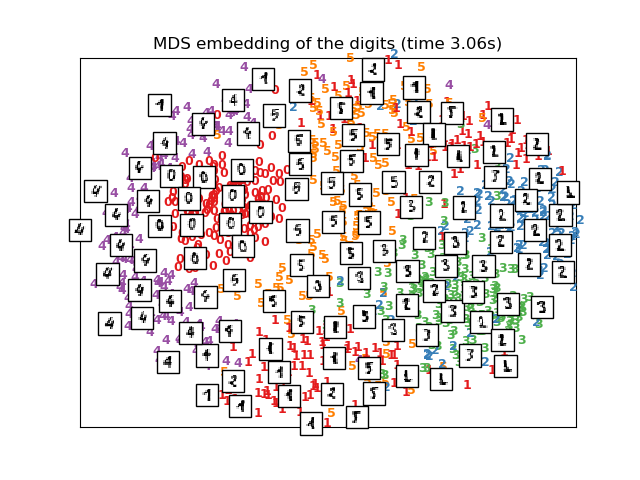
\includegraphics[width=0.9\textwidth]{img/digits_mds}
	\notesonly{\captionof{figure}{2D Embedding of the digits data using multi-dimensional scaling ``pairwise PCA''.}}
\end{center}
\end{minipage}
\begin{minipage}{0.47\textwidth}
\begin{center}
	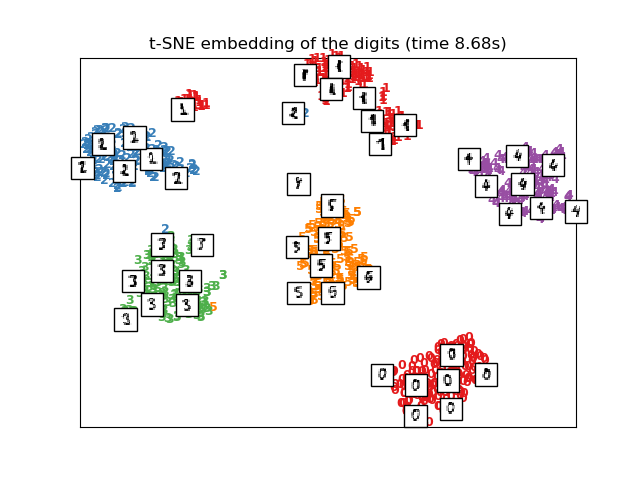
\includegraphics[width=0.95\textwidth]{img/digits_tsne}
	\notesonly{\captionof{figure}{2D Embedding of the digits data using t-SNE.}}
\end{center}
\end{minipage}

\notesonly{
Embedding figures for digits data were obtained from \href{https://scikit-learn.org/stable/auto_examples/manifold/plot_lle_digits.html}{here}
}
\end{frame}

\mode*

\clearpage

%\section{References}
%\begin{frame}[allowframebreaks] \frametitle{References}
	%\scriptsize
	%\bibliographystyle{plainnat}
	%\bibliography{bibliography}
%\end{frame}

\end{rightcolumn}
\end{paracol}

\end{document}
